% Document class `report-template` accepts either project-plan or final-report option in
% []. This will change the title page as necessary.
\documentclass[project-plan]{report-template}
% \documentclass[final-report]{report-template}

% Packages I use in my report.
\usepackage{graphicx}
\usepackage{amsmath}
\usepackage{pgfgantt}
\usepackage{bm}

\usepackage{setspace}
\linespread{1.1}
\setlength{\parindent}{0pt}
\setlength{\parskip}{4pt}
% tables
\usepackage{booktabs}

% units
\usepackage{siunitx}

% chemical formula
\usepackage{chemformula}

% enumerate
\usepackage{enumerate}

% for subfigures
\usepackage{caption}
\usepackage{subcaption}

% colours
%\usepackage{xcolor} %already loaded in cls
\definecolor{orange}{RGB}{255,127,0}
\definecolor{cool_blue}{RGB}{0,62,116}
\definecolor{light_blue}{RGB}{212,239,252}
\definecolor{cool_blue}{RGB}{0,110,175}

%python colours
\definecolor{pyblue}{HTML}{1F77B4}
\definecolor{pyorange}{HTML}{FF7F0E}
\definecolor{pygreen}{HTML}{2CA02C}
\definecolor{pyred}{HTML}{D62728}

\definecolor{codegreen}{rgb}{0,0.6,0}
\definecolor{codegray}{rgb}{0.5,0.5,0.5}
\definecolor{codepurple}{rgb}{0.58,0,0.82}
\definecolor{backcolour}{rgb}{0.95,0.95,0.92}

\lstdefinestyle{mystyle}{
    backgroundcolor=\color{backcolour},
    commentstyle=\color{codegreen},
    keywordstyle=\color{magenta},
    numberstyle=\tiny\color{codegray},
    stringstyle=\color{codepurple},
    basicstyle=\ttfamily\footnotesize,
    breakatwhitespace=false,
    breaklines=true,
    captionpos=b,
    keepspaces=true,
    numbers=left,
    numbersep=5pt,
    showspaces=false,
    showstringspaces=false,
    showtabs=false,
    tabsize=2
}
\lstset{style=mystyle}

\usepackage{pgfgantt} % for Gantt Chart

\ganttset{calendar week text={Wk~\currentweek}}
\newganttchartelement{orangebar}{
    orangebar/.style={
        inner sep=0pt,
        draw=pyorange,
        fill=pyorange, 
        very thick%,
        %top color=white,
        %bottom color=pyorange!80
    },
    orangebar label font=\slshape,
    orangebar left shift=.1,
    orangebar right shift=-.1
}

\newganttchartelement{bluebar}{
    bluebar/.style={
        inner sep=0pt,
        draw=pyblue,
        very thick,
        fill=pyblue
        %top color=white,
        %bottom color=blue!80
    },
    bluebar label font=\slshape,
    bluebar left shift=.1,
    bluebar right shift=-.1
}

\newganttchartelement{greenbar}{
    greenbar/.style={
        inner sep=0pt,
        draw=pygreen,
        very thick,
        fill = pygreen
        %top color=white,
        %bottom color=green!80
    },
    greenbar label font=\slshape,
    greenbar left shift=.1,
    greenbar right shift=-.1
}

\newganttchartelement{redbar}{
    redbar/.style={
        inner sep=0pt,
        draw=pyred,
        very thick%,
        %top color=white,
        %bottom color=pyred!80
    },
    redbar label font=\slshape,
    redbar left shift=.1,
    redbar right shift=-.1
}

% Directory where I saved my figures.
\graphicspath{{./figures/}}

% Metadata used for the title page - please modify.
\university{Imperial College London}
\department{Department of Earth Science and Engineering}
\course{MSc in Applied Computational Science and Engineering}
\title{Enhancing Commodity Price Predictions: Advanced Machine Learning Models for Oil and Precious Metals Forecasting}
\author{Peifeng Tan}
\email{pt623@imperial.ac.uk}
\githubusername{acse-pt623}
\supervisors{Antony Sommerfeld\\
                Yves Plancherel}
\repository{https://github.com/acse-pt623/irp-pt623-external.git}

\begin{document}

\maketitlepage  % generate title page

% Abstract
\section*{Abstract}
Copper is an indispensable raw material in modern industry and is widely used in a variety of sectors, including power electronics, household appliances, transportation and energy, machinery manufacturing and construction. However, as copper is both a commodity and a financial product, its price forecasting becomes exceptionally complex. This study aims to improve copper price forecasting by considering a range of influencing factors, including global supply and demand, energy costs, financial indicators and related commodity prices. Traditional econometric models such as ARIMA and ARMA have limitations in capturing nonlinear features in price changes. Therefore, we explore advanced machine learning models such as LSTM and the attention mechanism transformer. inspired by the success of the attention mechanism transformer in the field of natural language processing and image processing, we propose to use a transformer-like model incorporating a multi-head attention mechanism to capture feature-level interdependencies. In addition, we will incorporate sentiment analysis information from social media to improve prediction accuracy. This approach aims to provide a more robust and interpretable model for copper price forecasting. In the future, it is hoped that this model can be applied to other commodity forecasts.
% Introduction section
\section{Introduction}
\subsection{Problem description}
Oil and metals are crucial raw material and strategic resource for national economic development and energy industry. As a kind of vital raw materials, metals find wide applications in power electronics, household appliances, transportation energy, machinery manufacturing, and construction.~\cite{zhong2019time, qu2019unfolding, han2022r} Especially, copper which is a key industrial raw material, the global demand for it has continued to increase worldwide. Its electrical conductivity in electrical equipment, corrosion resistance in construction and versatility in manufacturing make it an indispensable resource.

\noindent However, copper is more than just an industrial raw material. Its trading in the commodity market also gives it the attributes of a financial product. This has made the forcasting of copper prices more complicated and difficult to control. Various factors such as supply and demand in the market, political factors, economic policies, and speculative behaviors can affect the price fluctuation of copper, which increases the difficulty of price forecasting.

\subsection{Iterature review}
\noindent Based on the complexity of copper prices, this study will consider a variety of influencing factors to forecast market changes in copper prices. First, as a commodity, global supply and demand, as well as the cost of energy for smelting and production, will influence the medium- to long-term trend of non-ferrous metal prices. Specifically, we consider coal prices, gasoline prices, crude oil prices, and natural gas prices~\cite{behmiri2015role}.
Second, as a financial product, copper's price fluctuations are also influenced by a variety of financial factors. We will consider factors such as the U.S. dollar exchange rate, consumer indices, and price levels. These include the GDP and EURUSD exchange rates, price conditions in the LME and COMEX markets, the U.S. Dow Jones Industrial Average, the price of Brent crude oil, gold, silver and iron ore futures, as well as the U.S. Dollar Index, and the U.S. Dollar to Renminbi (USD/CNY) and Australian Dollar (USD/AUD) exchange rates~\cite{frankel2010determinants, ciner2017predicting}.
Finally, copper prices are also influenced by other related products such as aluminum prices, gold prices, lead prices, iron ore prices, zinc prices, tin prices, silver prices and nickel prices. Price fluctuations in these products tend to have a strong correlation with the price of copper. Specifically, we take into account price movements of other major commodities in the international markets as well as relevant financial indicators~\cite{ozdemir2022medium, BUNCIC20151}.

\noindent In the past, many researchers used econometric models such as ARIMA~\cite{Asteriou2016ARIMAMA} and ARMA~\cite{whittle1951hypothesis} to forecast copper prices. However, these linear models cannot effectively capture the nonlinear features in price changes. With the development of machine learning, researchers began to try to use models such as NARX~\cite{lin1996learning, diaconescu2008use}, but these models usually require predefined model structures and have certain limitations. Subsequently, machine learning methods such as ANN~\cite{ZHANG2021102189}, KNN~\cite{altman1992introduction, chen2007narx}, SVM~\cite{cortes1995support}, Gaussian processes~\cite{frigola2013integrated}, decision trees and random forests~\cite{breiman2001random, diaz2020random} have been applied to copper price prediction with good results. However, these methods also face the problem of not being able to effectively capture the pre- and post-relationships of time series.

\noindent In order to better solve the above problems, RNN was introduced into time series prediction~|cite{rumelhart1986learning}, but RNN suffers from the problem of gradient vanishing when dealing with long sequences~\cite{bengio1994learning}.LSTM network, as an improvement of RNN, can better capture long time dependencies and has achieved remarkable results in time series prediction~\cite{hochreiter1997long}. With further reference to models such as CNN-LSTM~\cite{shi2015convolutional, 10159241} and DA-LSTM~\cite{qin2017dualstage}, our first goal is to construct an LSTM network with a view to obtaining better prediction results.

\noindent Recently, attention mechanisms have achieved great success in the fields of natural language processing and image processing. Especially in the field of natural language processing, the emergence of Transformer~\cite{li2019enhancing, vaswani2017attention} has contributed to the epochal achievement of large language models such as GPT. Inspired by this, we plan to try to use a model similar to Transformer to handle time series forecasting of copper prices. We will innovatively try to use a multi-attention mechanism to extract feature-level interdependencies instead of focusing only on time-level dependencies refering on DA-LSTM~\cite{qin2017dualstage}.This will help to explain and understand the impact of individual factors on price.

\noindent In addition, this study also plans to use information from social media to assist in predicting copper prices. Referring to studies such as “Sentiment Analysis with LSTM - NLTK”~\cite{8848203}, we introduce the element of sentiment analysis into the model to analyze the tendency of sentiment on social media in order to further improve the accuracy of the prediction.

\subsection{Objectives}

1. \textbf{Data Selection and Factor Identification}:
   \begin{itemize}
      \item \textbf{Screening Data}: Identify and collect relevant datasets that influence copper prices.
      \item \textbf{Identifying Usable Factors}: Determine key factors affecting copper price fluctuations.
   \end{itemize}

2. \textbf{Model Construction}:
   \begin{itemize}
      \item \textbf{LSTM Model}: Develop and train an LSTM network for accurate copper price predictions.
      \item \textbf{Transformer Model}: Implement a Transformer-like model with a multi-head attention mechanism to capture feature-level interdependencies.
   \end{itemize}

3. \textbf{Sentiment Analysis Integration}:
   \begin{itemize}
      \item \textbf{Sentiment Analysis}: Integrate social media sentiment analysis to improve prediction accuracy.
   \end{itemize}

4. \textbf{Performance Comparison}:
   \begin{itemize}
      \item \textbf{Baseline Model Comparison}: Compare the performance of advanced models (LSTM and Transformer) with traditional models like ARIMA and ARMA.
      \item \textbf{Improvement Assessment}: Evaluate improvements in prediction accuracy over baseline models.
   \end{itemize}

By achieving these objectives, the study aims to develop a robust and accurate model for predicting copper prices.

\begin{figure}[h]
    \centering
    \begin{subfigure}[b]{0.45\textwidth}
        \centering
        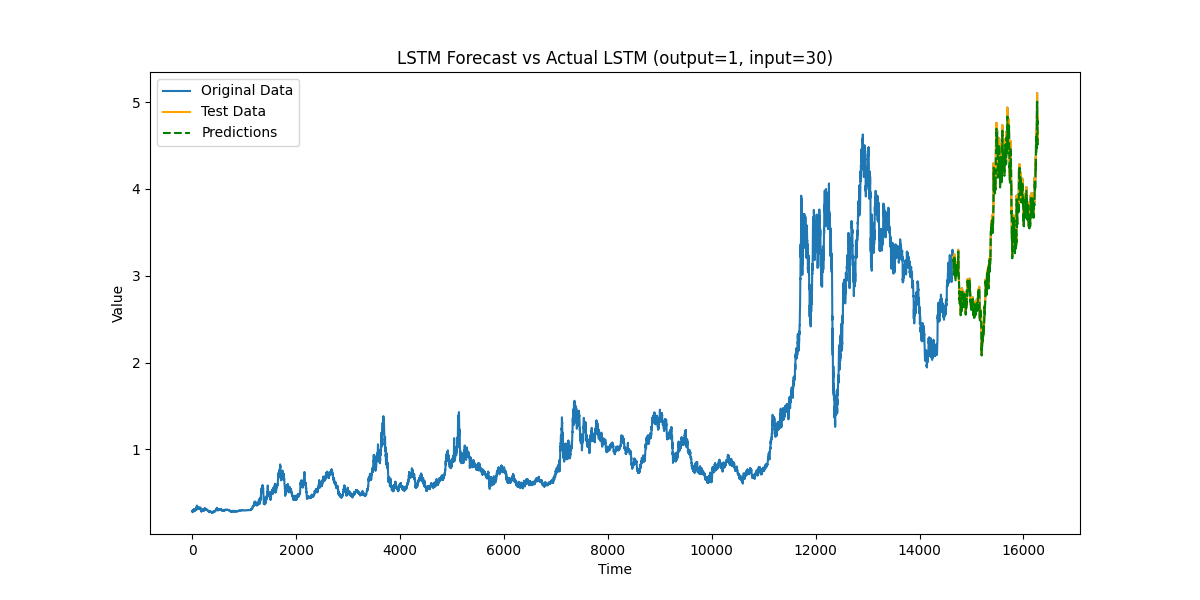
\includegraphics[width=\textwidth]{LSTM.png}
        \caption{LSTM}
        \label{fig:image1}
    \end{subfigure}
    \hfill
    \begin{subfigure}[b]{0.45\textwidth}
        \centering
        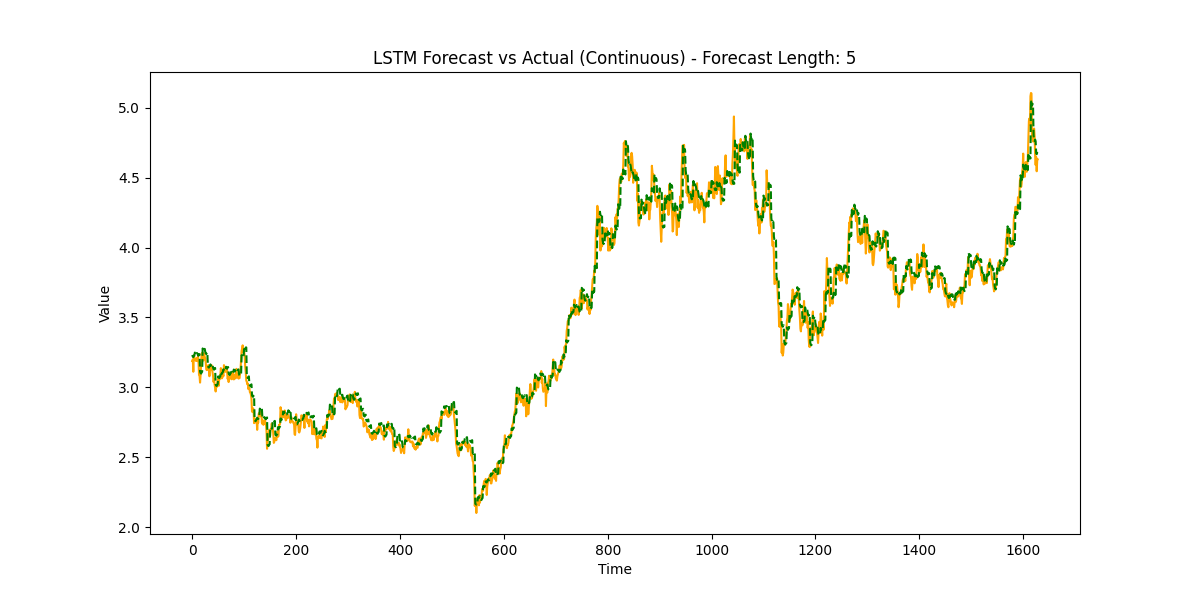
\includegraphics[width=\textwidth]{LSTM_zoomed.png}
        \caption{LSTM zoomed}
        \label{fig:image2}
    \end{subfigure}

    \vskip\baselineskip

    \begin{subfigure}[b]{0.45\textwidth}
        \centering
        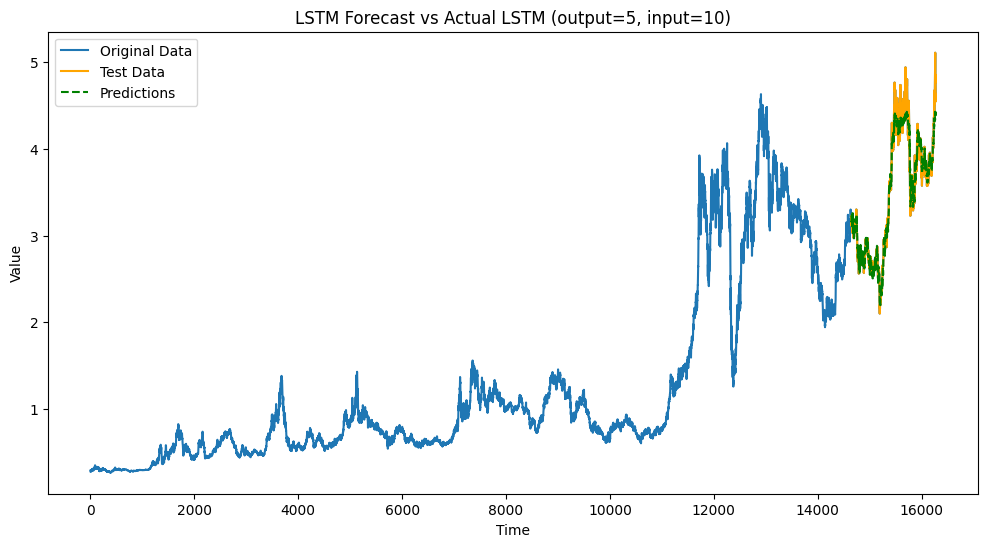
\includegraphics[width=\textwidth]{transformer.png}
        \caption{Transformer}
        \label{fig:image3}
    \end{subfigure}
    \hfill
    \begin{subfigure}[b]{0.45\textwidth}
        \centering
        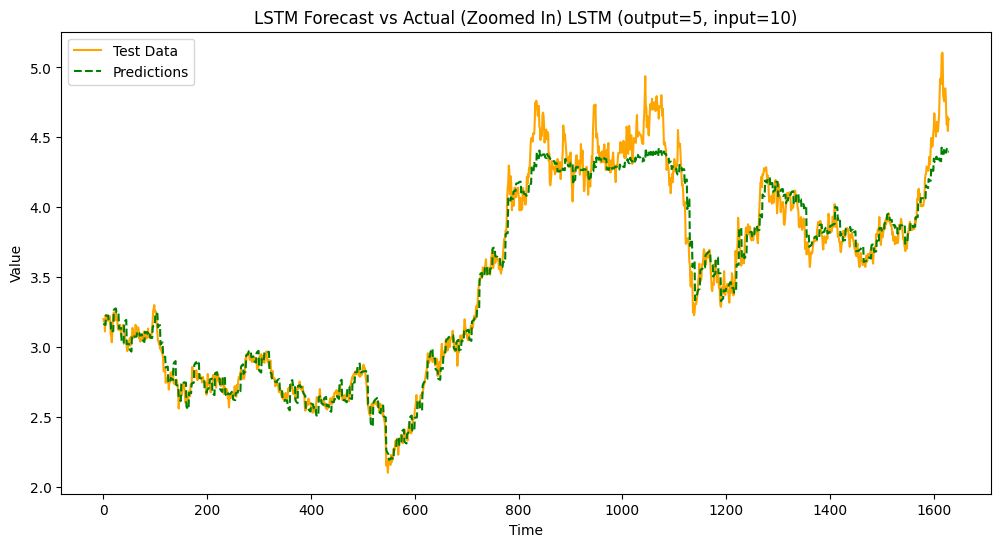
\includegraphics[width=\textwidth]{transformer_zoomed.png}
        \caption{Transformer zoomed}
        \label{Transformer zoomed}
    \end{subfigure}

    \caption{Performance of LSTM and Transformer in only price dataset}
    \label{fig:four_images}
\end{figure}

\section{Progress date}
\begin{enumerate}
    \item \textbf{Data collection:} The data collection phase has been completed, with access to a variety of data sources related to copper prices.
        
    \item \textbf{Feature engineering:} Based on the exploratory data analysis, feature engineering was performed, including feature selection, missing value processing, and data cleaning.
    
    \item \textbf{LSTM model construction:} Based on the only previous price data, an LSTM model has been constructed for copper price prediction, and the model has been trained and evaluated. It can be used to predict last week price.
    
    \item \textbf{Analysis of prediction results:} The prediction results of the LSTM model have been analyzed, including evaluating the accuracy and stability of the model and comparing it with the actual data.
    
    \item \textbf{Transformer model construction:} Try to construct the Transformer model for copper price prediction, explore its effect in time series prediction, and compare and analyze it with the LSTM model.

    \item \textbf{Comparison and analysis of results:} Compare and analyze the forecasting results of LSTM model and Transformer model, explore the advantages and disadvantages of both models, and put forward the corresponding conclusions and recommendations.

\end{enumerate}

\section{Future plan}
\begin{enumerate}
    \item \textbf{Exploratory Data Analysis (EDA):} Exploratory data analysis was conducted on the future collected data, including data distribution, outlier detection, and feature correlation analysis, etc, when garther more data.

    \item \textbf{Sentiment Analysis Model Integration:} Based on the prediction results, a sentiment analysis model is being integrated to consider the impact of social media sentiment on copper prices, and the model is being validated and evaluated.

    \item \textbf{Model Optimization:} Continue to optimize the LSTM model, including adjusting the model architecture, hyper-parameter optimization, etc., in order to improve the prediction effect.
    
    \item \textbf{Sentiment Analysis Model Improvement:} Improve the Sentiment Analysis Model, consider more social media data and sentiment features, and integrate them into the copper price prediction model.
            
    \item \textbf{Project Summary and Report:} Write a summary report of the project, including data collection, model construction, analysis of the experimental results, etc., and prepare presentation materials.
    
    \item \textbf{Possible Extended Research:} Explore the application of the model to the forecasting of other commodities or consider the influence of other external factors on the forecasting of copper prices, and provide directions for future research.
\end{enumerate}

\resizebox{\textwidth}{!}{
\begin{ganttchart}[
    hgrid style/.style={black, dotted},
    vgrid style/.style={*5{black,dotted}, *1{black, dotted}, *1{black, dashed}},
    x unit=2.3mm,
    y unit chart=9mm,
    y unit title=10mm,
    time slot format=isodate,
    group label font=\bfseries \small,
    link/.style={->, thick}
    ]{2024-05-27}{2024-08-30}
    \gantttitlecalendar{year, month=name, week}\\

    \ganttgroup[
        group/.append style={fill=orange}
    ]{Current Progress}{2024-05-27}{2024-07-10}\\ [grid]
    \ganttorangebar[
        name=DataCollection
    ]{Data Collection}{2024-05-27}{2024-06-05}\\ [grid]
    \ganttorangebar[
        name=EDA
    ]{Exploratory Data Analysis (EDA)}{2024-06-06}{2024-06-12}\\ [grid]
    \ganttorangebar[
        name=LSTM
    ]{LSTM Model Construction}{2024-06-13}{2024-06-19}\\ [grid]
    \ganttorangebar[
        name=Transformer
    ]{Transformer Model Construction}{2024-06-19}{2024-06-26}\\ [grid]
    \ganttorangebar[
        name=PredictionAnalysis
    ]{Analysis of Prediction Results}{2024-06-27}{2024-06-28}\\ [grid]
    \ganttorangebar[
        name=SentimentAnalysis
    ]{Sentiment Analysis Model Integration}{2024-07-04}{2024-07-6}

    \ganttnewline[thick, black]

    \ganttgroup[
        group/.append style={fill=blue}
    ]{Future Plan}{2024-07-6}{2024-08-30} \\[grid]
    \ganttbluebar[
        name=ModelOptimization
    ]{Model Optimization using other dataset}{2024-07-6}{2024-07-20}\\ [grid]
    \ganttorangebar[
        name=FeatureEngineering
    ]{Feature Engineering}{2024-07-6}{2024-06-10}\\ [grid]
    \ganttbluebar[
        name=SentimentImprovement
    ]{Sentiment Analysis Model Improvement}{2024-07-6}{2024-07-13}\\ [grid]
    \ganttbluebar[
        name=Develop model
    ]{Develop model and try others}{2024-07-13}{2024-08-10}\\ [grid]
    \ganttbluebar[
        name=Comparison
    ]{Comparison and Analysis of Results}{2024-08-10}{2024-08-19}\\ [grid]
    \ganttbluebar[
        name=Report
    ]{Project Summary and Report}{2024-08-20}{2024-08-30}
    
\end{ganttchart}
}

% References
\bibliographystyle{plain}
\bibliography{references}  % BibTeX references are saved in references.bib

\end{document}   